%保存为UTF-8编码格式
%用xelatex编译
 
\documentclass[UTF8,a4paper,12pt]{ctexart}
\usepackage[left=2.50cm, right=2.50cm, top=2.50cm, bottom=2.50cm]{geometry} %页边距
\CTEXsetup[format={\Large\bfseries}]{section} %设置章标题字号为Large,居左
%\CTEXsetup[number={\chinese{section}}]{section}
%\CTEXsetup[name={(,)}]{subsection}
%\CTEXsetup[number={\chinese{subsection}}]{subsection}
%\CTEXsetup[name={(,)}]{subsubsection}
%\CTEXsetup[number=\arabic{subsubsection}]{subsubsection}  %以上四行为各级标题样式设置,可根据需要做修改
 
%\linespread{1.5} %设置全文行间距
 
% \usepackage[backend=bibtex]{biblatex} 

\bibliographystyle{plain}
%\usepackage[english]{babel}
%\usepackage{float}     %放弃美学排版图表
\usepackage{fontspec}   %修改字体
\usepackage{amsmath, amsfonts, amssymb} % 数学公式相关宏包
\usepackage{color}      % color content
\usepackage{graphicx}   % 导入图片
\usepackage{subfigure}  % 并排子图
\usepackage{url}        % 超链接
\usepackage{bm}         % 加粗部分公式,比如\bm{aaa}aaa
\usepackage{multirow}
\usepackage{booktabs}
\usepackage{epstopdf}
\usepackage{epsfig}
\usepackage{longtable}  %长表格
\usepackage{supertabular}%跨页表格
\usepackage{algorithm}
\usepackage{algorithmic}
\usepackage{changepage}
\usepackage{listings}
\usepackage{xcolor}
\usepackage{booktabs}
\usepackage{enumitem}

 
 
%%%%%%%%%%%%%%%%%%%%%%%
% -- text font --
% compile using Xelatex
%%%%%%%%%%%%%%%%%%%%%%%
% -- 中文字体 --
%\setCJKmainfont{Microsoft YaHei}  % 微软雅黑
%\setCJKmainfont{YouYuan}  % 幼圆
%\setCJKmainfont{NSimSun}  % 新宋体
%\setCJKmainfont{KaiTi}    % 楷体
\setCJKmainfont[AutoFakeBold=true]{SimSun}   % 宋体
%\setCJKmainfont{SimHei}   % 黑体
 
% -- 英文字体 --
\setmainfont{Times New Roman}
%\setmainfont{DejaVu Sans}
%\setmainfont{Latin Modern Mono}
%\setmainfont{Consolas}
%
%
\renewcommand{\algorithmicrequire}{ \textbf{Input:}}     % use Input in the format of Algorithm
\renewcommand{\algorithmicensure}{ \textbf{Initialize:}} % use Initialize in the format of Algorithm
\renewcommand{\algorithmicreturn}{ \textbf{Output:}}     % use Output in the format of Algorithm
\renewcommand{\abstractname}{\textbf{\large {引\quad 言}}} %更改摘要二字的样式
\newcommand{\xiaosi}{\fontsize{12pt}{\baselineskip}}     %\xiaosi代替设置12pt字号命令,不加\selectfont,行间距设置无效
\newcommand{\wuhao}{\fontsize{10.5pt}{10.5pt}\selectfont}
 
\usepackage{fancyhdr} %设置全文页眉、页脚的格式
\pagestyle{fancy}
\lhead{}           %页眉左边设为空
\chead{}           %页眉中间
\rhead{}           %页眉右边
%\rhead{\includegraphics[width=1.2cm]{1.eps}}  %页眉右侧放置logo
\lfoot{}          %页脚左边
\cfoot{\thepage}  %页脚中间
\rfoot{}          %页脚右边
 
 
%%%%%%%%%%%%%%%%%%%%%%%
%  设置水印
%%%%%%%%%%%%%%%%%%%%%%%
%\usepackage{draftwatermark}         % 所有页加水印
%\usepackage[firstpage]{draftwatermark} % 只有第一页加水印
% \SetWatermarkText{Water-Mark}           % 设置水印内容
% \SetWatermarkText{\includegraphics{fig/ZJDX-WaterMark.eps}}         % 设置水印logo
% \SetWatermarkLightness{0.9}             % 设置水印透明度 0-1
% \SetWatermarkScale{1}                   % 设置水印大小 0-1
 
\usepackage{hyperref} %bookmarks
\hypersetup{colorlinks, bookmarks, unicode} %unicode
 
\lstset{
  basicstyle=\ttfamily\normalsize,
  keywordstyle=\mathcal,
  numbers=left,
  numberstyle=\tiny,
  frame=single,
  breaklines=true,
  backgroundcolor=\color{gray!10},
  keywordstyle=\color{blue}\bfseries,
  commentstyle=\color{orange!50!black},
  stringstyle=\color{red!50!black},
} 
 
\title{\textbf{\Large{车辆租赁管理系统实验报告}}}
\author{ 林杰泓 22336137 \\刘艺凡 22336162}
%\date{\today}
%\date{2021/10/21}
 
 
 
\begin{document}
 
\maketitle

\begin{abstract}
本任务关注设计车辆租赁管理系统,设计目的在于为用户和管理人员提供一个功能全面、操作便捷的车辆租赁平台,既能满足用户快速获取租车服务的需求,也能帮助管理人员在后台轻松实现对租车业务的高效管理
租车系统有三大核心的要求,车辆信息管理、租赁管理、客户管理。(1) 车辆信息管理要求记录和维护所有车辆的基本信息、租赁状态以及被租赁信息。 (2) 租赁管理要求对租车订单的创建、查询、修改等功能,需要能够高效处理订单状态。 (3) 客户管理要求对客户的基本信息、租车信息等数据进行管理,确保客户信息的安全性和准确性。
此外,车辆租赁管理系统还需要提供良好的交互页面,注重用户交互的便捷,确保前端与数据库之间的数据交互高效可靠。同时,系统需要设计合理的权限管理机制,确保客户与管理员能够在各自权限范围内安全使用系统数据。

在车辆租赁管理系统的设计中,我们采用Django Web框架作为后端技术栈,使用PostgreSQL作为数据库管理系统的信息,采用HTML,CSS,JavaScript框架开发前端交互页面。由于条件限制,本系统只支持本地部署。该系统开发人员为刘艺凡~(22336162)和林杰泓~(22336137)。系统需求分析,结构设计及功能模块设计由本组开发人员共同分析设计。
并由林杰泓负责用户信息管理及用户租赁管理的前端和后端开发和设计,由刘艺凡负责车辆信息管理和车辆信息管理的前端和后端的设计和开发。系统交互页面的设计及优化由两人共同完成。同时,我们共同负责了系统的安全性设计,包括对用户,车辆信息的保护,以及对用户,管理员的权限设置及授权。

我们在附件中提供了开发系统的相关代码。同时,为了便于查看和了解该车辆租赁管理系统的成果,我们提供了demo——\textbf{demo.gif},展示了该系统的功能。
此外,为了方便本地部署该系统,我们提供脚本\textbf{init.sh}用于构建简化对系统数据库的构建,同时也提供了 \textbf{README.md}作为指引,讲述部署系统以及使用系统的方法。更进一步的,当系统部署成功后,我们可以通过访问链接\href{http://127.0.0.1:8000/management/register}{http://127.0.0.1:8000/management/register} 进入系统的注册页面,以用户的视角开始体验该车辆租赁管理系统。

\end{abstract}

% \tableofcontents
 
% \begin{abstract}
% 本模板可以提供一般性单栏文档的生成,可以根据需要选择是否要目录、摘要,可自行选择日期生成方式,参考文献使用交叉引用条目形式使用,便于编辑和管理。务必注意,latex编译器需要选择xelatex.
% \end{abstract}
 
% \begin{center}
% \large{\textbf{Abstract}}
% \end{center}
 
% \begin{adjustwidth}{1cm}{1cm}
% \hspace{1.5em}Here is the first par. of abstract.Here is the first par. of abstract.
 
% \noindent\hspace{1.5em}Here is the second par. of abstract.Here is the second par. of abstract.
% \end{adjustwidth}
 
%\thispagestyle{empty}       %本页不显示页码
%\newpage                    %分页
%%\tableofcontents\thispagestyle{empty}
%\newpage
%\setcounter{page}{1}        %从下面开始编页,页脚格式为导言部分设置的格式


\newpage 
\tableofcontents
\newpage
\section{实验题目}
设计一个车辆租赁管理系统,包括车辆信息管理、租赁管理、客户管理等功能。车辆信息管理负责车辆
信息的添加、修改和查询;租赁管理负责租赁信息的录入、修改和查询;客户管理负责客户信息的添
加、修改和查询。
\section{概要设计}
\subsection{需求分析}

\subsubsection{功能需求}

\begin{itemize}
    \item 车辆信息管理:包括车辆的添加、修改、查询。每辆车有编号、品牌、型号、车牌号、租金等信息。
    \item 租赁管理:包括租赁记录的管理,租赁客户、租赁车辆等。
    \item 客户管理:管理客户信息,包含客户ID、姓名、联系方式等。
\end{itemize}

\subsubsection{非功能需求}

\begin{itemize}
    \item 安全性:对用户的权限进行控制,确保只有管理员可以进行修改操作。
    \item 系统响应时间:保证系统能快速响应用户操作,尤其是查询操作。
    \item 界面友好性:设计直观的用户界面,保证用户能够方便地操作和管理信息。
\end{itemize}

% \section{系统设计}

\subsection{系统结构}

\begin{figure}[htbp]  % figure 环境用于插入图片并进行浮动
    \centering  % 图片居中
    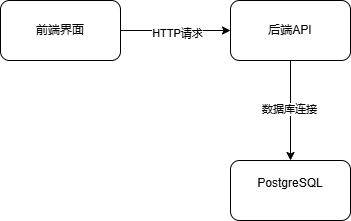
\includegraphics[width=1\textwidth]{pic/sap.png}  % 设置图片宽度为文档宽度的一半
    \caption{系统结构图}  % 图片标题
    \label{fig:sap}  % 图片标签,便于引用
\end{figure}

车辆租赁管理系统采用分层架构设计,
主要分为表现层、业务逻辑层和数据访问层,各层次的功能和作用如下:

\begin{itemize}
    \item 表现层(前端):\\
    表现层是系统与用户交互的部分,负责用户界面的显示和操作处理,
    包括车辆信息的查询、客户信息录入、租赁信息的修改等功能。
    具体技术采用HTML、CSS等前端技术,确保界面美观和用户体验友好。
    \item 业务逻辑层(后端):\\
    业务逻辑层位于表现层与数据访问层之间,
    是系统功能实现的核心部分,主要负责接收前端请求、
    处理业务逻辑并与数据库交互。车辆管理、租赁管理和客户管理的功能均在该层实现。
    本系统采用Django框架开发业务逻辑层,
    支持高效的请求响应和模块化开发。
    
    \item 数据访问层(数据库):\\
    数据访问层是系统的数据存储和管理部分,负责与数据库交互,
    执行SQL查询操作以实现数据的增删改查。
    本系统选用PostgreSQL作为数据库管理系统,
    设计了满足第三范式(3NF)的数据库结构,确保数据存储的规范性和完整性。
\end{itemize}

各层通过接口进行数据交互:表现层将用户请求发送给业务逻辑层,
业务逻辑层根据功能需求调用数据访问层与数据库交互,
最终返回结果至表现层供用户查看和操作。
这种分层设计提升了系统的可维护性和扩展性。

针对需求分析,我们得到了系统结构图,如图\ref{fig:sap}所示。

\subsection{系统功能模块}

\begin{figure}[htbp]  % figure 环境用于插入图片并进行浮动
    \centering  % 图片居中
    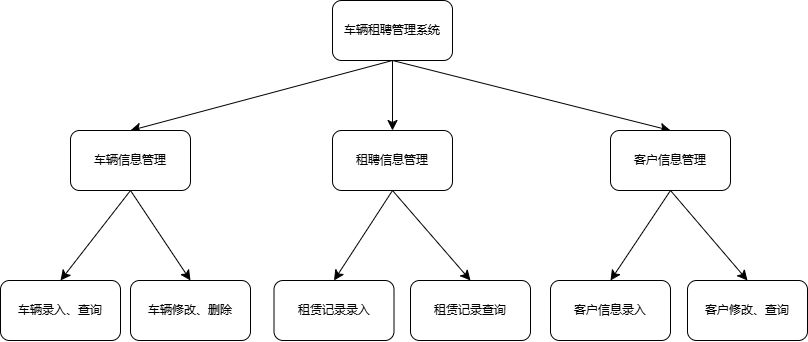
\includegraphics[width=1\textwidth]{pic/system_function_modules.png}  % 设置图片宽度为文档宽度的一半
    \caption{系统功能模块图}  % 图片标题
    \label{fig:sfm}  % 图片标签,便于引用
\end{figure}

车辆租赁管理系统的功能模块图以系统需求为基础,分为三个主要功能模块:
车辆信息管理模块、
租赁管理模块和客户信息管理模块。各模块的功能和相互关系描述如下:

% \vspace{-0.3cm}
\begin{itemize}
    \item 车辆信息管理模块:实现车辆信息的添加、修改等功能。\\
    添加功能用于录入车辆基本信息,如车辆编号、车型、租赁价格等。\\
    修改功能用于更新车辆状态或属性,如车辆的租赁状态、等。
    \item 租赁管理模块:实现租赁交易的管理,包括租赁信息的录入、修改和查询。\\
    录入功能记录租赁交易信息,如租赁车辆、客户、起始日期、结束日期及费用等。\\
    修改功能允许调整租赁的相关信息,如租赁时间或费用的变更。\\
    查询功能支持客户查找租赁记录,方便查看历史交易。
    \item 客户信息管理模块:实现客户信息的管理,包括添加、修改和查询功能。\\
    添加功能用于录入新客户的信息,如姓名、联系方式、身份证号等。\\
    修改功能用于更新客户信息,如更改联系方式或地址。\\
    查询功能支持按客户姓名或其他条件检索客户信息,便于用户管理客户数据。\\
\end{itemize}
\vspace{-0.8cm}
针对需求分析,我们得到了系统的功能模块图,如图\ref{fig:sfm}所示。

\section{详细设计}

\subsection{E-R图}

\begin{figure}[htbp]  % figure 环境用于插入图片并进行浮动
    \centering  % 图片居中
    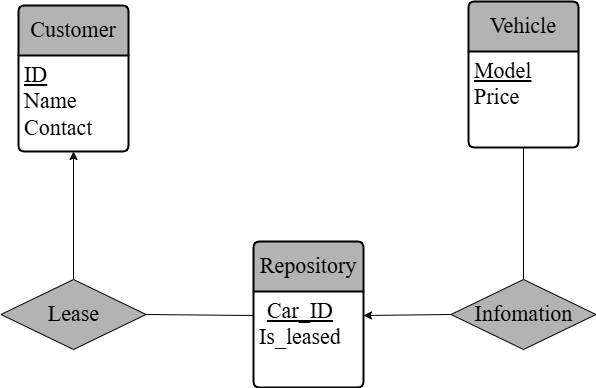
\includegraphics[width=1\textwidth]{pic/er.png}  % 设置图片宽度为文档宽度的一半
    \caption{E-R图}  % 图片标题
    \label{fig:er}  % 图片标签,便于引用
\end{figure}

车辆租赁管理系统的E-R图描述了系统中的主要实体及其之间的关系,
反映了系统的数据结构和逻辑关系~\cite{silberschatz2011database}。根据系统需求分析,设计了以下实体及其属性:

\subsubsection{实体及属性}

\begin{itemize}[leftmargin=0.3cm]
% \begin{itemize}
    \item 客户(Customer)属性:\\
    用户(User):与Django的内置用户模型进行一对一关联,扩展用户信息。\\
    ID(主键):客户唯一标识符。\\
    姓名(name):客户姓名。\\
    联系方式(contact):客户的联系方式。\\
\vspace{-0.7cm}
    \item 车辆(Vehicle)属性:\\
    型号(Model,主键):车辆的唯一标识。\\
    价格(Price):车辆的租赁价格。\\

    \item 车辆库(Repository)属性:\\
    车辆ID(Car\_ID,主键):标识库中每辆车的唯一编号。\\
    是否租赁(Is\_leased):表示车辆是否已被租赁。\\
\vspace{-0.7cm}
    \item 车辆信息(Info)属性:\\
    车辆ID(Car\_ID,外键):引用车辆库中的车辆ID。\\
    型号(Model,外键):引用车辆表中的型号信息。\\
\vspace{-0.7cm}    
    \item 租赁记录(Lease)属性:\\
    车辆ID(Car\_ID,外键):关联车辆库中的车辆。\\
    客户ID(ID,外键):关联客户表中的客户。\\
\end{itemize}

\subsubsection{实体之间的关系} 
\begin{itemize}[leftmargin=0.3cm]
\item 客户与租赁记录:
一个客户可以进行多次租赁记录(一对多)。

\item 车辆与车辆库:
车辆库中的每辆车属于一个车辆型号(多对一)。

\item 车辆库与租赁记录:
每辆车在租赁记录中最多出现一次(一对一)。

\item 车辆库与车辆信息:
每辆车在车辆信息表中有对应的详细记录(一对一)。
\end{itemize}
针对需求分析,画出E-R图表示的概念模型,如图\ref{fig:er}所示。

\subsection{数据库模式}




根据车辆租赁管理系统的需求和 E-R 图,将概念模型转换为关系模型,设计出满足第三范式(3NF)的数据库模式。具体如下:

\subsubsection{表设计}


\begin{table}[h!]
    \centering
    \caption{客户表(Customer)}
\begin{tabular}{|l|l|l|l|}
\hline
字段名 & 数据类型 & 约束 & 说明 \\
\hline
ID & VARCHAR(10) & PRIMARY KEY & 客户唯一标识符 \\
\hline
user\_id & INTEGER & UNIQUE, NOT NULL & 关联 Django 用户表 \\
\hline
name & VARCHAR(50) & NOT NULL & 客户姓名 \\
\hline
contact & VARCHAR(15) & NOT NULL & 客户联系方式 \\
\hline
\end{tabular}
\end{table}


\begin{table}[h!]
    \centering
    \caption{车辆表(Vehicle)}
\begin{tabular}{|l|l|l|l|}
\hline
字段名 & 数据类型 & 约束 & 说明 \\
\hline
Model & VARCHAR(50) & PRIMARY KEY & 车辆型号 \\
\hline
Price & INTEGER & NOT NULL & 租赁价格 \\
\hline
\end{tabular}
\end{table}


\begin{table}[h!]
    \centering
    \caption{车辆库表(Repository)}
\begin{tabular}{|l|l|l|l|}
\hline
字段名 & 数据类型 & 约束 & 说明 \\
\hline
Car\_ID & VARCHAR(10) & PRIMARY KEY & 车辆唯一标识符 \\
\hline
Is\_leased & BOOLEAN & DEFAULT FALSE & 是否被租赁 \\
\hline
\end{tabular}
\end{table}


\begin{table}[h!]
    \centering
    \caption{车辆信息表(Info)}
\begin{tabular}{|l|l|l|l|}
\hline
字段名 & 数据类型 & 约束 & 说明 \\
\hline
Car\_ID & VARCHAR(10) & FOREIGN KEY (Repository.Car\_ID), NOT NULL & 关联车辆库表 \\
\hline
Model & VARCHAR(50) & FOREIGN KEY (Vehicle.Model), NOT NULL & 关联车辆型号 \\
\hline
\end{tabular}
\end{table}


\begin{table}[h!]
    \centering
    \caption{租赁记录表(Lease)}
\begin{tabular}{|l|l|l|l|}
\hline
字段名 & 数据类型 & 约束 & 说明 \\
\hline
ID & VARCHAR(10) & FOREIGN KEY (Customer.ID), NOT NULL & 关联客户表 \\
\hline
Car\_ID & VARCHAR(10) & FOREIGN KEY (Repository.Car\_ID), NOT NULL & 关联车辆库表 \\
\hline
\end{tabular}
\end{table}

\subsubsection{数据库模式特点}

\begin{enumerate}
    \item \textbf{满足第三范式(3NF)}
    \begin{itemize}
        \item 消除冗余:每个表只存储一种实体的属性,避免数据冗余。
        \item 数据依赖明确:所有非主键字段完全依赖于主键。
    \end{itemize}
    \item \textbf{完整性约束}
    \begin{itemize}
        \item 主键约束:每个表都有明确的主键,保证数据唯一性。
        \item 外键约束:通过外键建立表间关系,保证数据一致性。
    \end{itemize}
    \item \textbf{扩展性}
    \begin{itemize}
        \item 模块化表设计便于功能扩展,如增加车辆维修管理、客户等级管理等功能。
    \end{itemize}
\end{enumerate}


\subsection{安全性与完备性}


为了确保车辆租赁管理系统的数据库安全性与完备性,采取了以下设计和实现措施:

\subsubsection{用户认证与权限管理}
\begin{itemize}
    \item \textbf{用户认证}:通过 Django 内置的用户认证系统(Authentication System),对系统用户进行登录验证,确保只有授权用户能够访问系统。
    \item \textbf{权限控制}:基于角色分配权限,不同用户(如管理员和普通用户)拥有不同的数据库访问权限。例如:
    \begin{itemize}
        \item 管理员:拥有添加、修改、删除数据的权限。
        \item 普通用户:仅能查看车辆信息和提交租赁请求。
    \end{itemize}
\end{itemize}

\subsubsection{数据完整性约束}
\begin{itemize}
    \item \textbf{主键约束}:每张表都有主键,确保每条记录具有唯一标识符。
    \item \textbf{外键约束}:外键关系保证了数据的一致性,例如租赁记录表中的车辆 ID 和客户 ID 必须合法且存在。
    \item \textbf{非空约束}:关键字段(如客户姓名、联系方式等)设置为非空,确保数据完整。
    \item \textbf{默认值约束}:为布尔字段(如车辆是否租赁)设置默认值,减少人为错误。
\end{itemize}

\subsubsection{数据保护与加密}
\begin{itemize}
    \item \textbf{敏感数据加密}:对于用户的敏感信息(如密码),使用 Django 提供的密码哈希功能进行加密存储。
\end{itemize}

Django 的 User 模型已经内置了密码哈希功能,
因此只需要使用 create\_user 或 set\_password 方法来处理用户密码。
下面是我们实现的思路:

\begin{lstlisting}[language=python]
    # 创建用户并加密密码
    user = User.objects.create_user(username=username, password=password)
\end{lstlisting}

\subsubsection{日志记录与审计}
\begin{itemize}
    \item 系统记录所有数据库操作的日志,包括数据添加、修改、删除等关键操作。
    \item 日志可用于追踪用户操作行为,及时发现和响应潜在的安全威胁。
\end{itemize}

\begin{lstlisting}[language=python]
    LOGGING = {
    'version': 1,
    'disable_existing_loggers': False,
    'formatters': {
        'verbose': {
            'format': '{levelname} {asctime} {module} {message}',
            'style': '{',
        },
        'simple': {
            'format': '{levelname} {message}',
            'style': '{',
        },
    },
    'handlers': {
        'console': {
            'level': 'DEBUG',
            'class': 'logging.StreamHandler',
            'formatter': 'simple',
        },
        'file': {
            'level': 'INFO',
            'class': 'logging.FileHandler',
            'filename': 'myapp.log',
            'formatter': 'verbose',
        },
    },
    'loggers': {
        'django': {
            'handlers': ['console'],
            'level': 'DEBUG',
            'propagate': True,
        },
        'myapp': {
            'handlers': ['console', 'file'],
            'level': 'DEBUG',
            'propagate': True,
        },
    },
}
\end{lstlisting}

在views.py中,我们可以记录用户操作日志,如下所示:

\begin{lstlisting}[language=python]
    if User.objects.filter(username=username).exists():
            logger.warning(f"Username {username} already exists.")
            messages.error(request, 'Username already exists. Please choose another one.')
            return render(request, 'management/register.html')
\end{lstlisting}

然后我们操作后就可以在myapp.log文件中看到相关日志。

\begin{lstlisting}[language=bash]
    WARNING 2024-12-25 10:36:47,223 views Username demo already exists.
    INFO 2024-12-25 10:41:41,707 views User demo logged in successfully.
    INFO 2024-12-25 10:41:43,616 views User demo returned vehicle with ID XPENG001.
    INFO 2024-12-25 10:41:54,603 views User demo returned vehicle with ID XPENG001.
\end{lstlisting}

\subsubsection{最小权限原则}
\begin{itemize}
    \item 数据库账户的权限设置遵循最小权限原则,只赋予完成任务所需的最低权限,避免权限过高导致的安全隐患。
\end{itemize}

通过以上安全性设计,系统能够有效保护数据免受未授权访问、篡改或丢失,确保数据库的完整性、保密性和可用性。

\section{调试与运行结果}
\subsection{问题与调试}
\subsection{最终结果展示}
经过精细的设计,我们实现了具备有注册登录功能的全面的租车管理系统。

\section{总结}
\bibliography{custom}
\end{document}

